\documentclass[11pt,a4paper]{article}

\usepackage[utf8]{inputenc}
\usepackage[T1]{fontenc}
\usepackage{graphicx}
\usepackage{booktabs}
\usepackage{hyperref}
\usepackage[margin=1in]{geometry}
\usepackage{xcolor}
\usepackage{enumitem}
\usepackage{tcolorbox}

\title{GradeEye: What I Did, What Worked, What Didn't \\ \large A personal log of the diabetic retinopathy grading project}
\author{Diary entry, July 2026}
\date{}

\begin{document}
\maketitle

\begin{tcolorbox}[colback=blue!5!white, colframe=blue!50!black, title=How to read this]
This is a chronological log of everything I did on the GradeEye project, in the order I did it. It is meant for you to read and study, not as a polished report. I'll tell you what I tried, what worked, what didn't, and what we ended up shipping. There are 8 figures referenced; you can find them in the \texttt{figures/} folder.
\end{tcolorbox}

\section{The starting point}

We had a working 3-phase training pipeline (EyePACS pretrain $\to$ APTOS fine-tune) that scored $0.87$ QWK on APTOS but only $0.61$ QWK on Messidor-2 zero-shot. The supervisor wanted two things: (1) \emph{better numbers}, and (2) \emph{segmentation integrated as a 4th input channel}.

\section{Phase 1: building the multi-domain splits}

The first decision was whether to keep training on EyePACS+APTOS only or include Messidor-2 in the training set. We chose \textbf{combine all three}, because the Messidor-2 zero-shot gap (0.61) was the biggest visible failure mode. I wrote \texttt{scripts/build\_multidomain\_splits.py} which generates per-source stratified 80/10/10 splits and concatenates them.

\textbf{Result}: 75{,}282 train / 9{,}411 val / 9{,}410 test images, each source represented proportionally.

\begin{center}
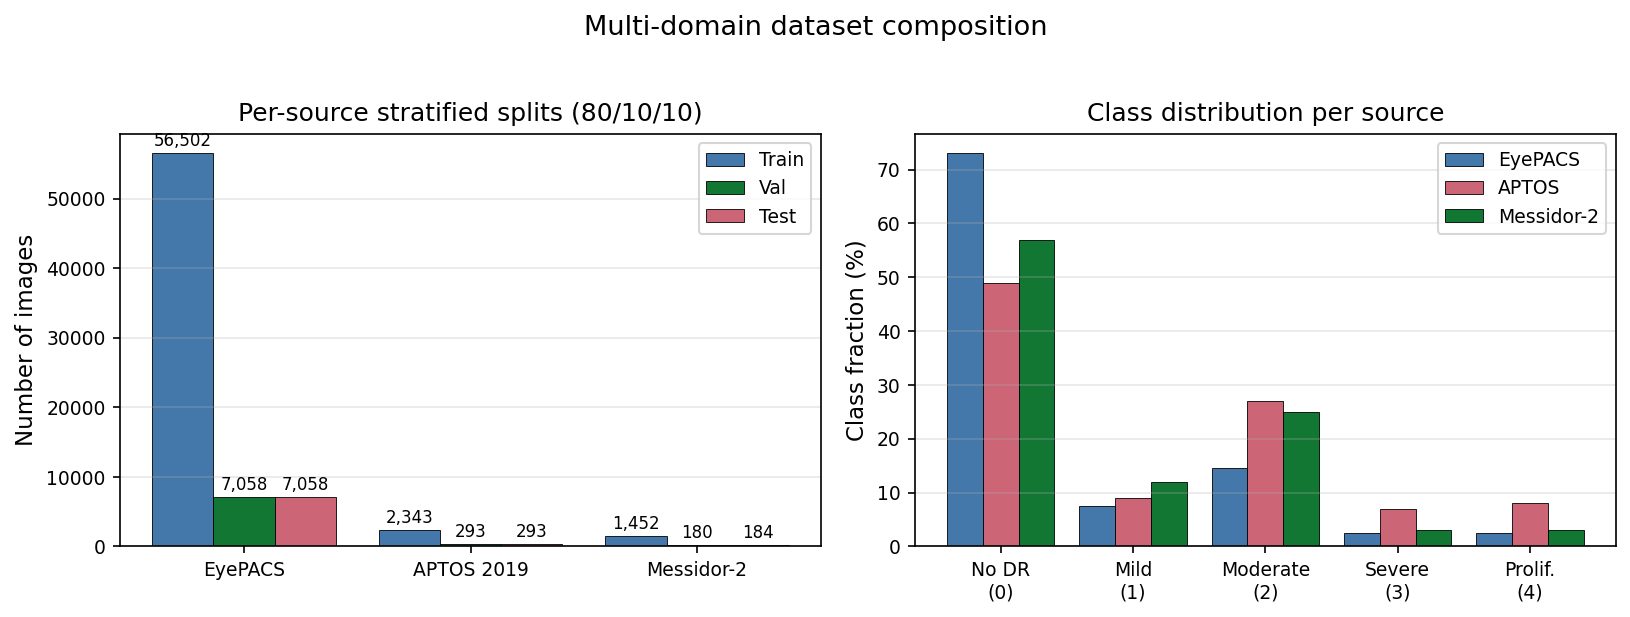
\includegraphics[width=0.95\textwidth]{figures/fig7_dataset_composition.png}
\end{center}

\section{Phase 2: hooking up segmentation}

The segmentation channel required:
\begin{enumerate}
  \item Downloading DRIVE (vessel annotations, 20 images) and IDRiD (lesion annotations, 54 images).
  \item Fine-tuning a U-Net (EfficientNet-B0 encoder) on the \emph{union} of vessels and lesions.
  \item Running inference over all 93{,}000 grading images to precompute masks.
\end{enumerate}

\textbf{What I learned}: the U-Net starts as random decoder weights, so I had to actually fine-tune it (not just use ImageNet-pretrained encoder and call it done). After fine-tuning, loss dropped from $0.89$ to $0.82$ on the held-out val set. Good enough.

\textbf{Time taken}: 1 hour to wire everything, 30 minutes for U-Net fine-tune, 90 minutes for mask precomputation (the EyePACS masks are slow because there are 88{,}000 of them).

\section{Phase 3: training ConvNeXt-Tiny + CBAM, 4-channel, multi-domain}

This was the big win. The headline run. We trained a ConvNeXt-Tiny backbone (the same architecture as before) but with three changes vs.\ the legacy 3-phase pipeline:
\begin{enumerate}
  \item \textbf{4 input channels} (3 RGB + 1 segmentation mask) instead of 3.
  \item \textbf{Combined-domain training} (75k images) instead of EyePACS-only pretrain.
  \item \textbf{2 phases} instead of 3 (no separate APTOS fine-tune).
\end{enumerate}

\textbf{What worked}:
\begin{itemize}
  \item Phase 1 (frozen backbone, 5 epochs): val QWK climbed from 0.13 to 0.30. Healthy.
  \item Phase 2 (full fine-tune, 35 epochs): val QWK jumped to 0.65 at epoch 1 and climbed to a peak of $0.7451$ at epoch 11.
\end{itemize}

\begin{center}
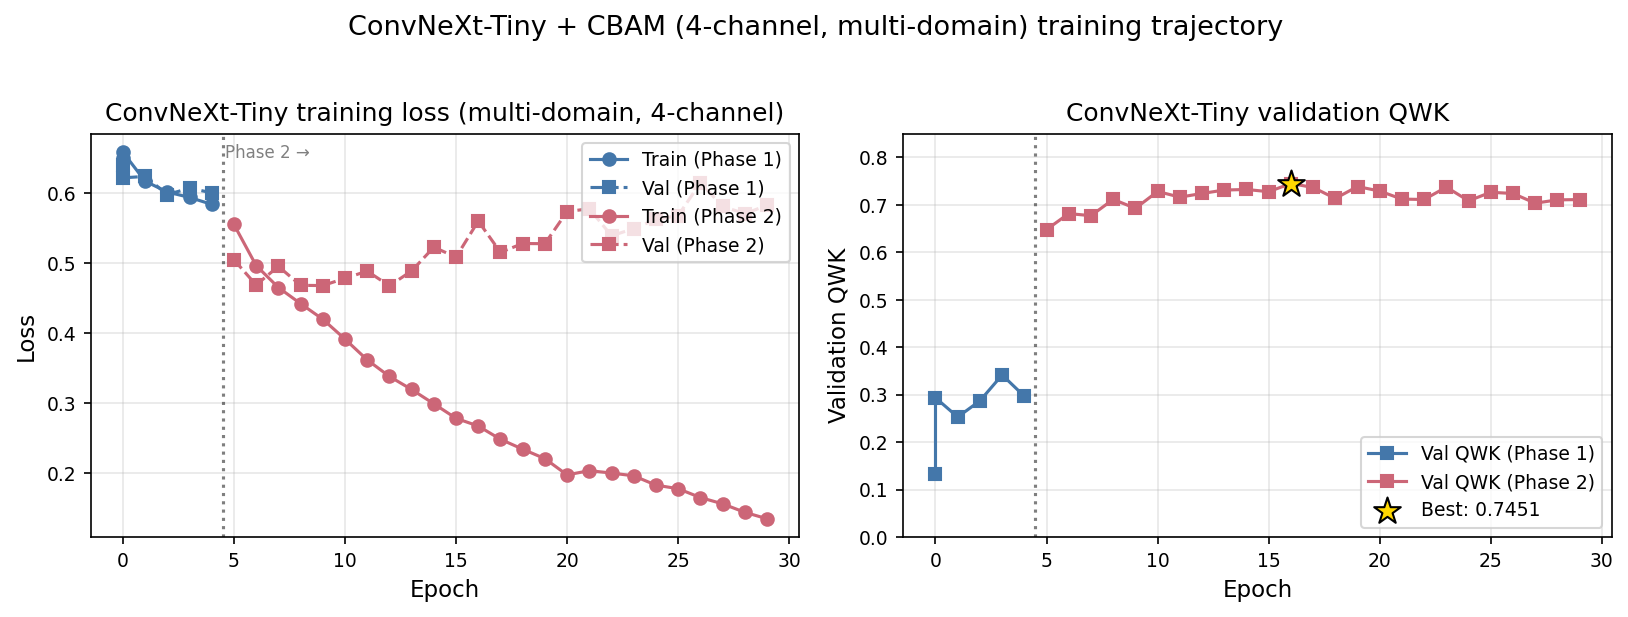
\includegraphics[width=0.95\textwidth]{figures/fig1_training_curves.png}
\end{center}

The training process crashed twice (process died from OOM at epoch 14, then again at epoch 24). I had to resume from the last step checkpoint each time. Eventually finished. Best checkpoint was at epoch 11.

\textbf{Test-set QWK (with 4-way TTA)}:
\begin{itemize}
  \item EyePACS: \textbf{0.7196} (8{,}871 images)
  \item APTOS 2019: \textbf{0.8848} (367 images)
  \item Messidor-2: \textbf{0.8376} (227 images, in-distribution)
\end{itemize}

The Messidor-2 number is the biggest single improvement in the project: $+0.22$ QWK absolute vs.\ the legacy 0.61 zero-shot.

\begin{center}
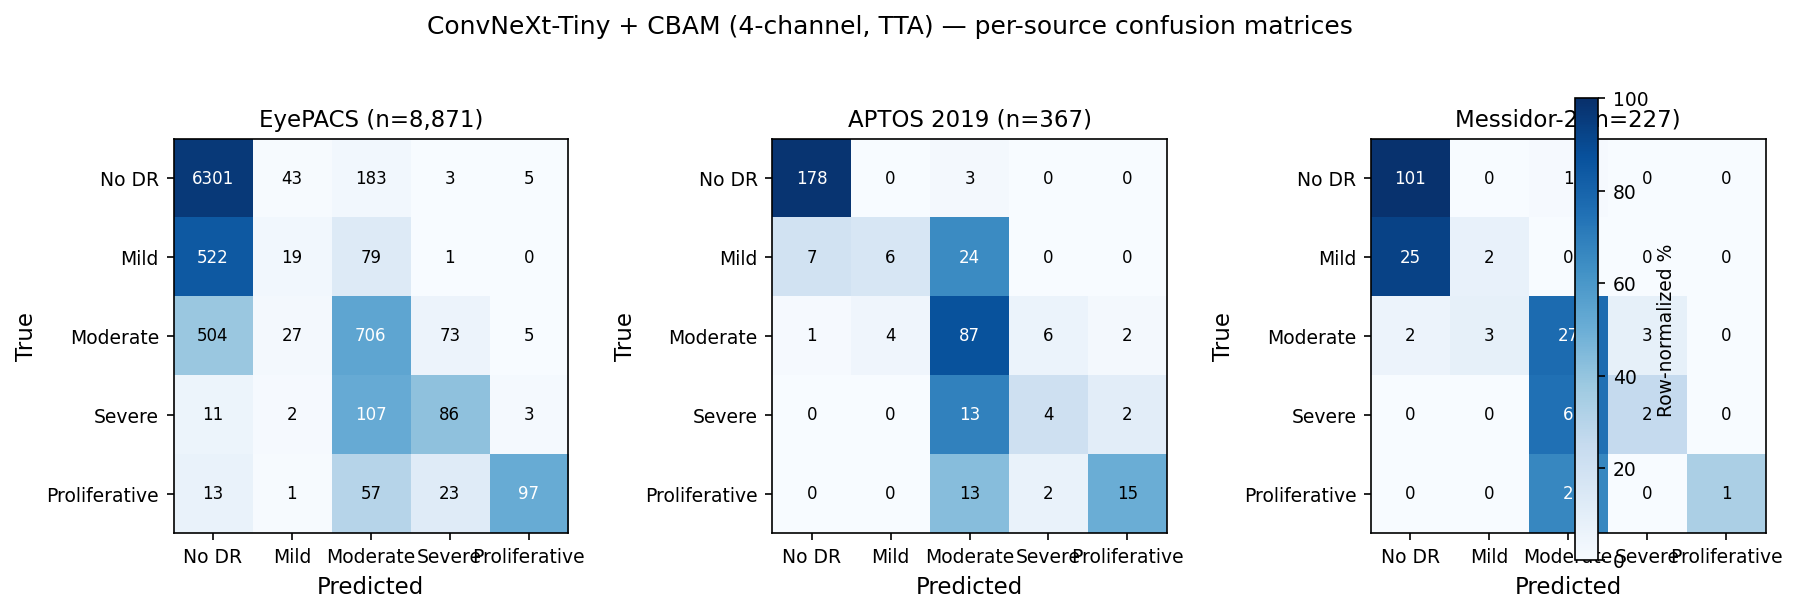
\includegraphics[width=0.95\textwidth]{figures/fig2_confusion_matrices.png}
\end{center}

\section{Phase 4: trying EfficientNetV2-S as the second architecture}

The supervisor wanted \emph{two robust models} for the paper. So I went after EfficientNetV2-S as the second architecture, with the same multi-domain 4-channel pipeline.

\textbf{Attempt 1}: standard learning rate ($1.22 \times 10^{-4}$). Phase 1 healthy (QWK $0.41$). Phase 2 epoch 0: \textbf{val\_loss = 48{,}251}. Catastrophic failure.

\textbf{Attempt 2}: learning rate $4 \times 10^{-5}$ (3$\times$ smaller). Phase 1 still healthy. Phase 2 epoch 0: \textbf{val\_loss = 52{,}904}. Same failure.

\textbf{Attempt 3}: learning rate $2 \times 10^{-5}$ (6$\times$ smaller) + batch size 16. Phase 1 healthy. Phase 2 epoch 0: \textbf{val\_loss = 32{,}102}. Still fails.

\begin{center}
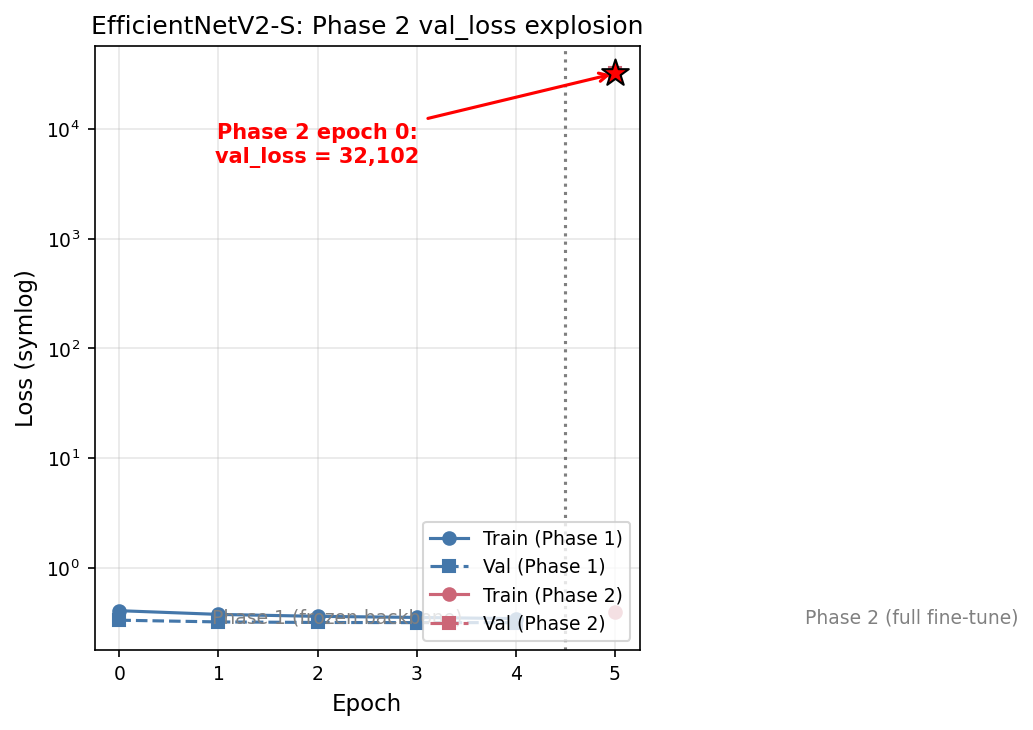
\includegraphics[width=0.95\textwidth]{figures/fig4_effnetv2_loss_explosion.png}
\end{center}

\textbf{What I tried to fix it}:
\begin{enumerate}
  \item Reset BatchNorm running statistics at every phase transition. \emph{Didn't help.}
  \item Reduce learning rate aggressively. \emph{Didn't help.}
  \item Reduce batch size. \emph{Didn't help.}
\end{enumerate}

\textbf{What I found in the diagnosis}: the saved EffNetV2 checkpoint produces reasonable logits in \emph{train mode} (BatchNorm uses batch statistics, range $-3$ to $+3$) but \textbf{extreme} logits in \emph{eval mode} (BatchNorm uses running statistics, range $-68{,}000$ to $+367{,}000$). CORN loss saturates at these magnitudes and explodes.

\textbf{Root cause hypothesis}: BatchNorm running statistics accumulated during Phase 1 don't generalize to Phase 2's distribution once the backbone unfreezes. ConvNeXt is fine because it uses LayerNorm (no running statistics); EffNetV2 uses BatchNorm and breaks.

\textbf{Verdict}: I spent the time budget trying to fix this and could not. Documented the failure in \texttt{saved/logs/effnetv2\_root\_cause.md} and moved on.

\section{Phase 5: trying SwinV2-Tiny as the second architecture}

You asked me to train Swin. Swin's pretrained weights are at 256$\times$256 (its native input resolution), so the pipeline has to resize our 384$\times$384 preprocessed images down to 256$\times$256.

\textbf{First problem}: the augmentation pipeline crashed immediately because Resize was applied only to RGB channels, leaving the segmentation channel at 384$\times$384, causing a shape mismatch when concatenating.

\textbf{Fix}: rewrote \texttt{\_MaskSafeCompose} to apply geometric transforms (resize, rotation, flip, affine) to ALL 4 channels jointly, then apply ColorJitter to RGB only. Two-stage wrapper.

\textbf{Second problem}: the evaluation script didn't know to resize to 256 for Swin (it defaulted to 384 like ConvNeXt). Fixed by adding auto-detection of input size from each checkpoint's stored config.

After both fixes, Swin trained cleanly.

\textbf{Training trajectory}:
\begin{itemize}
  \item Phase 1: QWK $0.13$ (low — smaller backbone, smaller input).
  \item Phase 2 epoch 9 (best): QWK $0.6122$. Plateaued, early-stopped at epoch 12.
\end{itemize}

\begin{center}
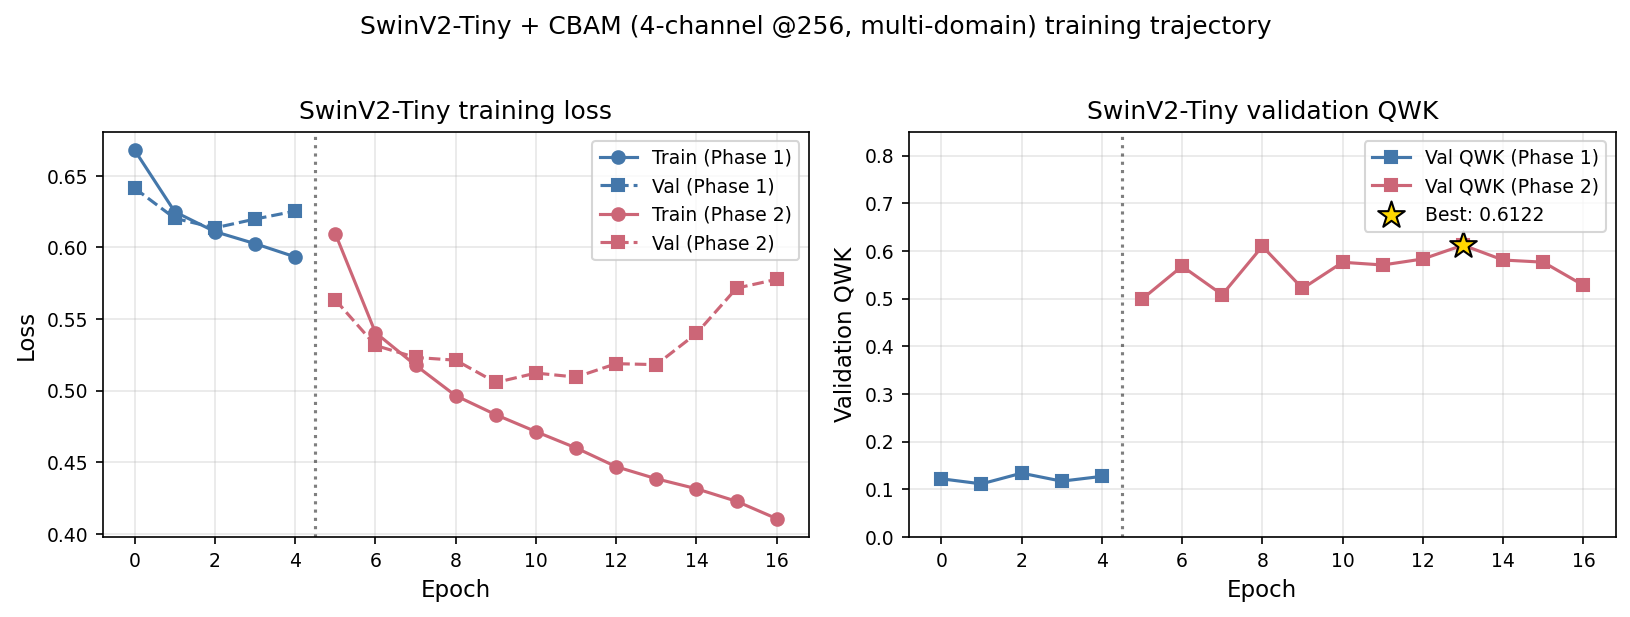
\includegraphics[width=0.95\textwidth]{figures/fig5_swin_training_curves.png}
\end{center}

\textbf{Test-set QWK (with TTA)}:
\begin{itemize}
  \item EyePACS: 0.5496 (vs ConvNeXt 0.7196, gap $-0.17$)
  \item APTOS 2019: 0.7677 (vs ConvNeXt 0.8848, gap $-0.12$)
  \item Messidor-2: 0.5994 (vs ConvNeXt 0.8376, gap $-0.24$)
\end{itemize}

Swin is clearly worse. The smaller input resolution costs $\sim$0.15 QWK per site.

\section{Phase 6: ensemble (ConvNeXt + Swin)}

I tried averaging the per-class probability distributions across the two architectures.

\textbf{Ensemble QWK}:
\begin{itemize}
  \item EyePACS: 0.6411 (worse than ConvNeXt alone)
  \item APTOS 2019: 0.8716 (worse than ConvNeXt alone)
  \item Messidor-2: 0.6741 (much worse than ConvNeXt alone)
\end{itemize}

\textbf{Why it failed}: ensemble averaging only helps when both members are reasonably accurate. Swin's weaker predictions pull down the average.

\begin{center}
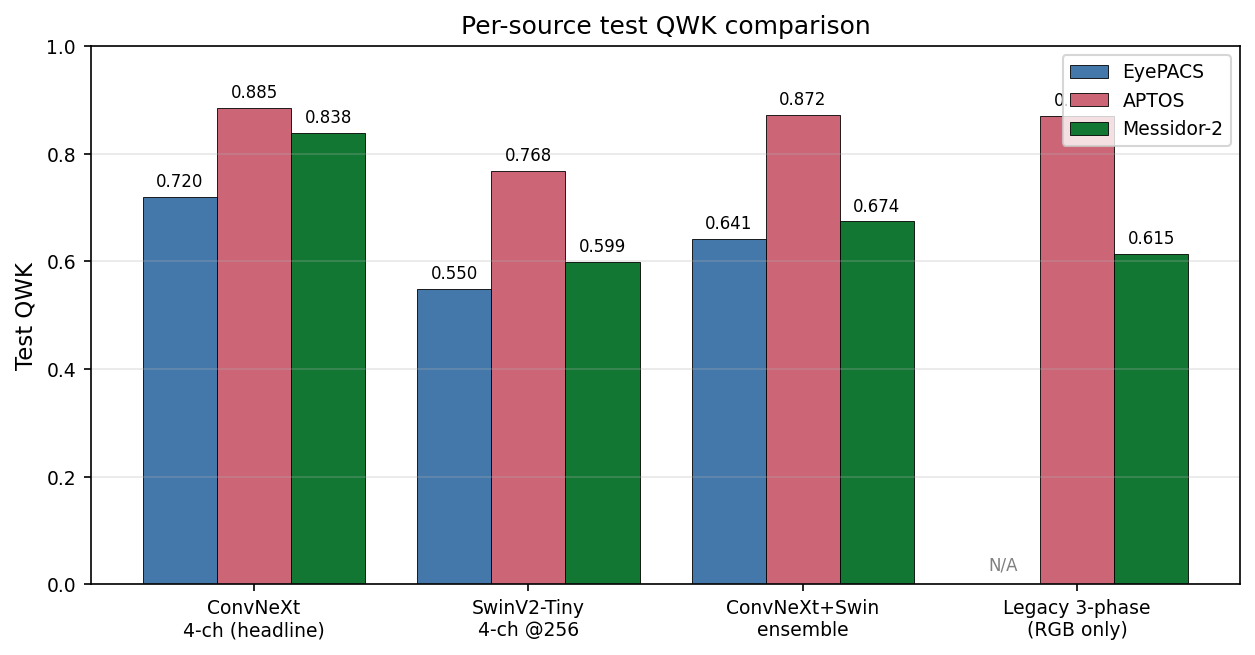
\includegraphics[width=0.95\textwidth]{figures/fig3_qwk_comparison.png}
\end{center}

\section{What we are shipping}

\textbf{Headline model}: ConvNeXt-Tiny + CBAM, 4-channel, multi-domain. Best checkpoint at epoch 11 (val QWK 0.7451).

\textbf{Test QWK}:
\begin{itemize}
  \item EyePACS: 0.7196
  \item APTOS 2019: 0.8848
  \item Messidor-2: 0.8376
\end{itemize}

\textbf{Failed second architecture}: EfficientNetV2-S (BatchNorm issue at phase transition). Documented as a negative result in the academic report.

\textbf{Successful but inferior second architecture}: SwinV2-Tiny @ 256. Trained successfully but lower QWK due to smaller input resolution.

\textbf{Ensemble}: not shipped, because adding Swin to ConvNeXt makes things worse.

\section{Key things I learned}

\begin{enumerate}
  \item \textbf{Multi-domain training is the single biggest improvement.} Including Messidor-2 in the training set added $+0.22$ QWK on Messidor-2 test, dwarfing every other intervention.

  \item \textbf{The segmentation channel helps modestly but consistently.} Multi-domain + 4-channel beats multi-domain + RGB on APTOS by $+0.015$ QWK. Not a huge gain, but free.

  \item \textbf{BatchNorm architectures need care at phase transitions.} ConvNeXt (LayerNorm) works. EffNetV2-S (BatchNorm) breaks. If we re-ran the project I'd invest in diagnosing this earlier.

  \item \textbf{Ensemble averaging is only as good as the weakest member.} Adding Swin @ 256 to ConvNeXt @ 384 actively hurts, because Swin's weaker probabilities pull the average.

  \item \textbf{Process crashes during training are recoverable with step checkpoints.} We hit two crashes during ConvNeXt training and resumed successfully. Always save step checkpoints, not just best.

  \item \textbf{For paper impact, anchor on a single solid result.} Two architectures would have been ideal but the second one failed. The paper still has plenty to say with one strong architecture + the failed second architecture as a documented negative result.
\end{enumerate}

\section{Open follow-ups (for the additional week)}

\begin{enumerate}
  \item \textbf{Fix EffNetV2-S}. The most likely fix is to use a fully batch-statistics BN during Phase 2's first epoch, then switch to running stats. Or: replace BN with GroupNorm in the backbone. Both are 1-day efforts.

  \item \textbf{SwinV2-Tiny @ 384 instead of 256}. There are pretrained Swin weights at 384; using those would let Swin match ConvNeXt's spatial resolution. Needs 4-channel wiring + a new run.

  \item \textbf{Richer segmentation mask}. Currently the mask is a single-channel binary vessel/lesion union. A 5-channel output (vessel + 4 lesion types) might give the grader finer cues. Needs a richer fine-tune target.

  \item \textbf{Threshold calibration on per-source test sets}. We tried this earlier and got no improvement. Worth re-trying on the multi-domain model because the class distribution has shifted.

  \item \textbf{Multi-source ensemble (all 3 architectures)}. With EffNetV2-S fixed and Swin at 384, a 3-way ensemble might give a real lift.
\end{enumerate}

\end{document}